\documentclass[10pt]{beamer}

\usetheme{metropolis}
\usepackage{appendixnumberbeamer}

\usepackage{booktabs}
\usepackage[scale=2]{ccicons}

\usepackage{pgfplots}
\usepgfplotslibrary{dateplot}

\usepackage{xspace}
\newcommand{\themename}{\textbf{\textsc{metropolis}}\xspace}

\title{Detecting Malicious Shell Commands}
\subtitle{A review of text classification techniques}
\date{\today}
\author{rdube}
% \institute{Center for modern beamer themes}
% \titlegraphic{\hfill\includegraphics[height=1.5cm]{logo.pdf}}


\begin{document}

\maketitle

\begin{frame}{Table of contents}
  \setbeamertemplate{section in toc}[sections numbered]
  \tableofcontents[hideallsubsections]
\end{frame}

\section{Motivation}

\begin{frame}[fragile]{Why study this topic?}
	Several reasons to study the topic:
	\begin{itemize}
		\item Powershell increasingly used in attacks \cite{symc2016}
		\item (In general) Fileless attack techniques increasing \cite{symc2017}
		\item Scripts becoming weapons of choice for sophisticated attack groups \cite{msft2017-2}
		\begin{itemize}
			\item Fileless technques used during the SolarWinds hack \cite{zdnet2021}
		\end{itemize}
		\item Complicated and obfuscated scripts difficult for human analysts to decipher \cite{feye2018}
	\end{itemize}
\end{frame}

\section{Input data source}

\begin{frame}{What input source to assume?}
	Techniques used, models created may be different based on input assumed \cite{msft2017-2,msft2019,feye2018}:
	\begin{itemize}
		\item PowerShell vs. VBScript vs. Javascript code 
		\item Single command line vs. multi-line script
		\item Raw script vs. that obtained through AMSI or sandbox
		\item Obfuscated vs. de-obfuscated script
		\item Additional unlabelled corpus of scripts
	\end{itemize}
\end{frame}

\section{Degree of pre-processing}

\begin{frame}[fragile]{What pre-processing to assume?}
	Prior work raises several quesions regarding pre-processing data \cite{powershell2018,amsi2019,feye2018}:
	\begin{itemize}
		\item Mechanism to declare a label malicious?
		\item De-obfuscate script coded in base64 (and other) encodings?
		\item Normalize scripts using different IP addresses?
		\item Normalize scripts using random file names?
		\item Normalize abbreviations?
		\item What demarcation to use between tokens?
		\item Eliminate rare tokens?
		\item De-duplicate scripts via clustering and representative selection?
	\end{itemize}
	But, pre-processing partially depends on the the type of model chosen
\end{frame}

\section{Model design space}

\begin{frame}[fragile]{What model design attributes to choose?}
	The model design space is large \cite{survey2021,msft2017,powershell2018,amsi2019,feye2018,feye2018-2,textcnn2016,textcnn2019}:
	\begin{itemize}
		\item Manual feature extraction (traditional classification) vs. automatic feature extraction (neural network)
		\item Character based model vs. token (word) based model?
		\item Bag-of-words vs. embedding representation?
		\item Inline embedding vs. separately trained embedding?
		\item Use CNN for feature extraction?
		\item (For sequnce modeling) LSTM vs Transformers? 
		\item (If multiple models are used) Ensemble technique to combine verdicts?
		\item (If other signals are used) Ensemble technique to include external signals?
	\end{itemize}
\end{frame}

\section{Understanding prior work}

\begin{frame}[fragile]{Extract coherent lego block models}
	\begin{itemize}
		\item textCNN model \cite{textcnn2016,textcnn2019,powershell2018}
		\item CNN-LSTM model \cite{amsi2019}
		\item Obfuscation detection model \cite{feye2018}
	\end{itemize}
\end{frame}

\begin{frame}[fragile]{Lego block model 1: textCNN}
	\begin{figure}
		\includegraphics[scale=0.28]{textcnn}
		\caption{Text CNN model as used in \cite{powershell2018}}
	\end{figure}
\end{frame}

\begin{frame}[fragile]{Lego block model 2: CNN-LSTM}
	\begin{figure}
		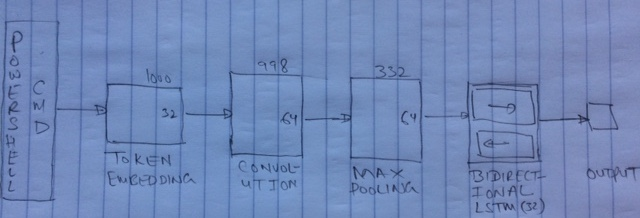
\includegraphics[scale=0.50]{cnn-lstm}
		\caption{CNN-LSTM model as used in \cite{amsi2019}}
	\end{figure}
\end{frame}

\begin{frame}[fragile]{Lego block model 3: obfuscation detection}
	\begin{figure}
		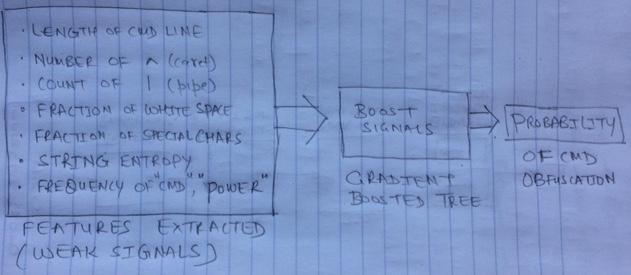
\includegraphics[scale=0.50]{gbtree}
		\caption{Obfuscation detection model as used in \cite{feye2018}}
	\end{figure}
\end{frame}

\begin{frame}[standout]
  Questions?
\end{frame}

\appendix

\begin{frame}[allowframebreaks]{References}

  \setbeamertemplate{bibliography item}{\insertbiblabel}
  \bibliography{cmd}
  \bibliographystyle{alpha}

\end{frame}

\end{document}
